% ICEIC 2027 -- English working draft v3, 2026-10-27.
% Based on conference_101719_lm8_repeat.tex (v2); title and author edits preserved.
% Source branch: exp/structured-k8-lm8-repeat.
% Matched PPL follow-up: b438a098c6025df1e6928fd2c504381dcffef448.
% Retained repeated timings: 565acc7b11076a1635fce7e076eb8cb9b4a27317.
% PPL: one teacher-forced pass/window/configuration on four REUSED reference
% windows (4092 targets/configuration); no new independent held-out evaluation.
% Performance: ten warmed measured sessions/configuration, kept separate.
% Compile with pdfLaTeX. No external figure or bibliography files are needed.
% Results are transcribed from the author's committed experiment reports;
% this drafting process did not rerun the device experiments.
% AUTHOR CHECK: confirm author order, official affiliations, email, funding,
% publication clearance, original logs, and all experimental descriptions.
\documentclass[conference,a4paper,10pt]{IEEEtran}
\usepackage{cite}
\usepackage{amsmath,amssymb}
\usepackage{graphicx}
\usepackage{booktabs}
\usepackage{url}
\usepackage{flushend}
\usepackage{tikz}
\usetikzlibrary{arrows.meta,positioning}
\newcommand{\fl}{\operatorname{fl}_{16}}
\newcommand{\clip}{\operatorname{clip}}
\hyphenation{quan-ti-za-tion de-quan-ti-za-tion code-book}

\begin{document}
\title{Structured KV Cache Quantization for Mobile NPUs}
% Replace this block after confirming ALL authors and the official affiliation.
% Add an approved funding acknowledgement only when its exact text is known.
\author{\IEEEauthorblockN{Jeongwoo Han}
\IEEEauthorblockA{\textit{Working draft: author list, affiliations, and contact information to be confirmed}}}
\maketitle

\begin{abstract}
Key--value cache quantization reduces storage requirements but can introduce substantial encoding and restoration overhead on mobile neural processing units. This paper presents a hardware-oriented implementation and evaluation of Structured K8, a two-region piecewise-uniform key quantizer with arithmetic indexing and a lookup-free Hexagon Vector eXtensions decoder. The design uses four shared coefficients and preserves explicit half-precision rounding. We integrate it into a mixed-precision cache with eight-bit keys in half of the layers, four-bit keys elsewhere, and two-bit values throughout. On a Galaxy S26 Ultra running Qwen3-1.7B in a W4A16 configuration, the cache occupies 28.875 MiB at a context capacity of 1024 tokens. Across ten warmed measurements per configuration, Structured K8 reduces mean time to first token by 32.62 percent and increases mean decoding throughput by 13.61 percent relative to converged Lloyd--Max under Odd placement; matched Boundary placement yields 31.12 percent and 14.41 percent, respectively. A separate teacher-forced evaluation on four previously used WikiText-2 windows finds 1.81 percent higher perplexity under Odd placement but 0.45 percent lower perplexity under Boundary placement, indicating placement-dependent quality ordering. A separate three-run uniform-quantizer comparison shows similar observed throughput and lower aggregate perplexity on a different held-out set. A same-codebook decoder probe records 39.56 percent fewer physical vector-unit busy cycles. These results support an implementation-level quality--efficiency trade-off within the tested conditions, not broad-domain or cross-device generalization.
\end{abstract}

\begin{IEEEkeywords}
KV cache, quantization, mobile NPU, piecewise-uniform quantization, Hexagon HVX
\end{IEEEkeywords}

\section{Introduction}
Autoregressive large language models retain attention keys and values in a key--value (KV) cache. Quantizing this cache can reduce its storage and data-transfer requirements, but effective deployment also depends on the cost of producing and consuming the compressed representation. KIVI illustrates the importance of treating key and value distributions differently~\cite{kivi}. TurboQuant studies random-rotation-based scalar quantization and distinguishes reconstruction error from inner-product distortion~\cite{turboquant}. Neither a nominal bit width nor a scalar distortion value alone determines the latency of a particular mobile implementation.

Our work builds upon a TurboQuant implementation integrated into the Qualcomm AI Hub Models inference pipeline~\cite{artifact}. Its Lloyd--Max (LM) encoder uses comparison trees and centroid-selection subgraphs; larger codebooks increase this graph-level work. On the decoder side, centroid lookup and layout conversion also consume accelerator resources. We investigate whether a restricted codebook can simplify both paths while retaining useful language-model quality.

Piecewise quantization is established prior art. PWLQ divides a distribution into regions with separate uniform grids~\cite{pwlq}, and PTQ4ViT introduces twin uniform quantization for vision-transformer activations~\cite{ptq4vit}. Building on these established ideas, our contribution is a hardware-oriented specialization for a rotated KV cache: an arithmetic encoder, a byte-compatible HVX decoder with an explicit numerical contract, and controlled on-device comparisons against converged LM and single-spacing uniform baselines. Mixed key/value precision and layer placement serve as deployment choices supporting this implementation.

\section{Structured Quantization and Implementation}
\subsection{Rotated, Norm-Corrected Cache Representation}
For a nonzero key vector $x\in\mathbb{R}^{d}$, the inherited codec computes
\begin{equation}
 n=\lVert x\rVert_2,\qquad y=R(x/n),
 \label{eq:rotation}
\end{equation}
where $R$ is a fixed orthogonal matrix and $d=128$. Dense QR-generated rotations use seeds 42 and 542 for keys and values, respectively; matrix generation occurs offline. The experiments retain norm correction and disable the quantized Johnson--Lindenstrauss (QJL) residual-correction stage. Thus, this implementation is not the full inner-product-unbiased TurboQuant construction~\cite{turboquant}.

Let $\hat c$ be the signed centroid vector selected for $y$. Conceptually, the effective scale and restored rotated coordinates are
\begin{equation}
 s_{\mathrm{eff}}=\fl\!\left(n/\lVert\hat c\rVert_2\right),
 \qquad \hat z_i=\fl(s_{\mathrm{eff}}\hat c_i).
 \label{eq:scale}
\end{equation}
Here $\fl$ denotes rounding to IEEE half precision. The implementation retains its existing guards and FP16 operation boundaries; zero vectors restore to zero through a zero scale. The surrounding attention rotation and layout policy is unchanged. The new native decoder produces scale-corrected rotated coordinates, rather than introducing a new attention algorithm.

\subsection{Two-Region Codebook and Arithmetic Indexing}
Structured K8 represents a magnitude by one region bit $r\in\{0,1\}$ and a six-bit local index $k\in\{0,\ldots,63\}$. Each region has offset $a_r$ and spacing $\Delta_r$. Its deployed positive centroid is
\begin{equation}
 c^+_{r,k}=\fl\!\left(\fl(k\Delta_r)+a_r\right).
 \label{eq:centroid}
\end{equation}
The negative half is obtained by sign reflection. Four shared coefficients are fitted offline by analytically integrated scalar mean-squared error (MSE) under $\mathcal{N}(0,1/128)$, with nine fixed initializations and ordering/positive-spacing constraints. No observed KV samples or model perplexity select these coefficients. This Gaussian model is a design approximation, not a claim about the exact empirical distribution or global optimality.

The frozen FP16 offsets are $a_0=0.00089263916015625$ and $a_1=0.1268310546875$; the spacings are $\Delta_0=0.001956939697265625$ and $\Delta_1=0.00376129150390625$. The region boundary $\tau$ is the midpoint between $c^+_{0,63}$ and $c^+_{1,0}$. For magnitude $m=|y_i|$, the logical index rule is
\begin{align}
 r &= \mathbf{1}[m>\tau], \nonumber\\
 k &= \clip\!\left(\left\lfloor (m-a_r)\Delta_r^{-1}+\tfrac12\right\rfloor,0,63\right).
 \label{eq:index}
\end{align}
Execution uses the stored reciprocal and explicit intermediate rounding, so this logical expression is not a cross-precision bit-exactness claim. Arithmetic ties follow the floor rule, not LM's lower-index tie convention.

Writing $j=64r+k$, the stored byte is
\begin{equation}
 b_i=\begin{cases}
 128+j,&y_i\geq0,\\
 127-j,&y_i<0.
 \end{cases}
 \label{eq:byte}
\end{equation}
This reflection preserves an ascending symmetric byte-to-centroid interface. Negative region/local fields must be reflected before decoding. Each coordinate is stored directly as UINT8; K8 requires no sub-byte packing. K4 and V2 still use their existing packed representations.

\begin{figure}[t]
\centering
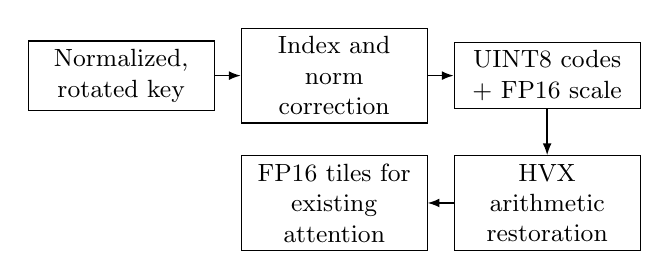
\begin{tikzpicture}[
 box/.style={draw,align=center,text width=2.15cm,minimum height=0.83cm,inner sep=3pt,font=\small},
 arr/.style={-{Latex[length=1.5mm]},line width=0.5pt},node distance=0.33cm]
 \node[box] (input) {Normalized,\\rotated key};
 \node[box,right=of input] (index) {Index and norm\\correction};
 \node[box,right=of index] (cache) {UINT8 codes\\+ FP16 scale};
 \node[box,below=0.58cm of cache] (hvx) {HVX arithmetic\\restoration};
 \node[box,left=of hvx] (tiles) {FP16 tiles for\\existing attention};
 \draw[arr] (input)--(index);
 \draw[arr] (index)--(cache);
 \draw[arr] (cache)--(hvx);
 \draw[arr] (hvx)--(tiles);
\end{tikzpicture}
\caption{Structured K8 path. The same frozen coefficients define encoding and restoration. Other key/value codecs and the attention layout remain unchanged.}
\label{fig:path}
\end{figure}

\subsection{HVX Decoder and Storage Budget}
The encoder is lowered to QNN HTP graph operations. The native HVX decoder extracts the magnitude code, selects a region's coefficients, reconstructs the centroid with separate FP16 multiply/add instructions, restores its sign, and multiplies by the effective scale. A 128-byte input load produces two 128-byte FP16 output vectors. The implementation avoids centroid-table loads and per-coordinate scalar loops. The coefficient payload is eight bytes, versus 512 bytes for an explicit 256-entry FP16 codebook; this is a codebook-storage comparison, not a measured total-memory reduction. Fusing the multiply and add would change the prescribed rounding and is not used.

Both tested placements assign K8 to 14 of Qwen3-1.7B's 28 layers, LM K4 to the other 14, and LM V2 throughout. \emph{Odd placement} uses zero-based layers $1,3,\ldots,27$; \emph{Boundary placement} uses layers $0$--$6$ and $21$--$27$. Each quantizer comparison uses the same mask within a placement. These names describe layer selection, not uniform scalar quantization. Average index precision is six bits for keys and two for values. With eight KV heads, dimension 128, and capacity 1024, the implementation allocates 28 MiB of indices and 0.875 MiB of FP16 scales, totaling 28.875 MiB. Both current and past KV are compressed, and restoration uses the existing 256-token tiles. This host-cache allocation excludes runtime I/O buffers, process memory, and accelerator scratch space.

\section{Experimental Methodology}
We use Qwen3-1.7B~\cite{qwen3} in a fixed W4A16 configuration on a Galaxy S26 Ultra (SM8850), using QAIRT 2.48.0.260626 and the HTP backend in burst mode. Inference uses a single sequence with context capacity 1024. Model weights, activation encodings, rotation seeds, norm correction, and K4/V2 paths are held fixed within each quantizer comparison; no weight training or activation recalibration is performed. The implementation and recorded experiments are identified by immutable commits~\cite{artifact}. Table~\ref{tab:lm-repeated} summarizes the repeated performance comparison.

\begin{table*}[t]
\caption{Repeated on-device performance with matched layer masks. Values are mean $\pm$ sample SD across ten measured sessions per configuration, excluding warm-up. Improvements denote lower TTFT or higher throughput relative to converged LM8, computed from group means. Every configuration allocates 28.875 MiB of host KV storage.}
\label{tab:lm-repeated}
\centering
\setlength{\tabcolsep}{8pt}
\begin{tabular}{@{}llrrr@{}}
\toprule
Placement & Metric & Converged LM8 & Structured K8 & Improvement (\%)\\
\midrule
Odd & TTFT (ms) & $745.990\pm11.668$ & $502.653\pm12.595$ & 32.62\\
 & Prefill (tokens/s) & $1203.854\pm19.009$ & $1787.642\pm44.911$ & 48.49\\
 & Decode (tokens/s) & $33.249\pm0.053$ & $37.775\pm0.232$ & 13.61\\
\midrule
Boundary & TTFT (ms) & $726.580\pm13.099$ & $500.487\pm9.512$ & 31.12\\
 & Prefill (tokens/s) & $1236.104\pm22.874$ & $1795.119\pm34.854$ & 45.22\\
 & Decode (tokens/s) & $33.101\pm0.051$ & $37.870\pm0.121$ & 14.41\\
\bottomrule
\end{tabular}
\end{table*}

Quality is teacher-forced perplexity on selected WikiText-2 documents~\cite{wikitext}. A 1024-token window has 1023 scored targets. Aggregate perplexity is $\exp(\sum_j\mathrm{NLL}_j/\sum_j N_j)$, where $\mathrm{NLL}_j$ is a window's summed negative log-likelihood. It is not an average of window perplexities or a full-corpus WikiText-2 result.

A separate quality follow-up evaluates the four unchanged binaries from Table~\ref{tab:lm-repeated} on the same four previously used WikiText-2 reference windows. The existing AR128 teacher-forced scorer runs once per window and configuration in a fresh process/session: 16 passes in total and 4092 scored targets per configuration. No warm-up, repeated scoring, logit dump, profiling, or generation-speed measurement is added. Host/device binary, runtime, configuration, and input hashes are checked against the performance experiment's frozen artifacts before and after scoring. These windows are reused references, not a new independent held-out test.

The earlier LM and uniform quality experiments also include four held-out documents each, fixed by content-hash order with exclusions for previously recorded titles and 16-token overlaps. Their held-out sets A and B differ, so absolute held-out PPL must not be compared across those experiments. Held-out status refers to those experiments, not pretraining. Neither held-out set is rescored in the follow-up; the earlier Odd-placement results remain separately labeled, and no matched Boundary held-out comparison is available.

Uninstrumented performance uses 897 prompt tokens and 128 generated tokens. The first generated token is produced during prefill; the subsequent 127 autoregressive (AR1) steps bring the cache to $897+127=1024$ tokens. Decode throughput is 127 divided by the summed durations of those steps. TTFT excludes model loading. Each invocation performs a full warm-up sequence, resets the KV cache, and then measures a second session on the same loaded model and input. Warm-up is excluded from the reported timing.

The repeated LM comparison covers four configurations: Structured and converged LM8 under Odd and Boundary placement. Ten counterbalanced rounds yield ten measured sessions per configuration, or 40 in total, plus 40 excluded warm-ups. Two Williams blocks and two reversed orders balance each pair's execution precedence five to five; each configuration occupies each within-round position two or three times. A fixed ten-second pause follows each invocation. All measured samples are retained, with no failures or replacements. We report means and sample standard deviations; improvements are ratios of group means, not averages of per-run ratios.

All four configurations use the same runner and Native package. Existing binaries are reused except for the missing Boundary converged-LM control, built before measurement. All 24 compiled AR1/AR128 graphs pass the I/O, rotation, and FP16-attention audit; paired non-codec initializers and activation encodings match. SHA-256 checks pass before and after measurement. No QNN optrace or detailed profiling is enabled. Current HAL temperatures and Android thermal status are sampled identically across configurations, spanning loading, warm-up, and measurement; they do not directly expose HTP clocks or throttling.

The earlier uniform comparison retains its three sessions per configuration in the order Uniform, Structured, Structured, Uniform, Uniform, Structured. Its timing, the earlier layer-placement study, and single-session codec probes remain separate experiments; their samples are not pooled with the new warmed LM measurements.

\section{Results and Analysis}
\subsection{Comparison with Converged Lloyd--Max}
LM100 is the inherited codebook generated with 100 Lloyd iterations; it is not a converged optimum. A stronger baseline runs four deterministic initializations until both centroid movement and relative MSE change satisfy strict convergence criteria for ten consecutive iterations. All four yield the same FP16 table. The minimum integrated Gaussian MSE falls from $1.3054680\!\times\!10^{-6}$ to $3.2175846\!\times\!10^{-7}$; Structured's nearest-centroid value is $4.7935449\!\times\!10^{-7}$. Hence Structured is not superior in scalar reconstruction error to converged LM.



Table~\ref{tab:lm-repeated} reports the repeated measurements. Under Odd placement, Structured reduces mean TTFT by 32.62\% and increases mean prefill/decode throughput by 48.49\%/13.61\% relative to converged LM8. Under Boundary placement, the corresponding changes are 31.12\%, 45.22\%, and 14.41\%. Thus, the observed performance advantage persists under both tested masks, but is not established for every placement. This comparison changes both encoder structure and decoder, measuring complete implementations rather than the decoder alone.

Supplemental paired-round bootstrap 95\% intervals for TTFT reduction are [31.51, 33.71]\% for Odd and [30.01, 32.23]\% for Boundary; decode-increase intervals are [13.23, 13.91]\% and [14.23, 14.57]\%, respectively. These small-sample, single-device intervals describe this experiment; shared thermal drift may affect them. Earlier single-session timings lacked the same-process warm-up and are not pooled with these results. No quantizer, kernel, or runner optimization was introduced by this repetition, so changes from historical absolute timings are not attributed to algorithm changes.

\begin{table}[t]
\caption{Matched reference-window quality follow-up using the unchanged performance binaries. One teacher-forced pass per window and configuration; 4092 scored targets per configuration. These four WikiText-2 windows are reused, not independently held out.}
\label{tab:lm-ppl}
\centering
\setlength{\tabcolsep}{4pt}
\begin{tabular}{@{}llrr@{}}
\toprule
Placement & K8 codec & Mean NLL & PPL $\downarrow$\\
\midrule
Odd & LM-conv. & 3.143864 & 23.19332\\
 & Structured & 3.161763 & 23.61219\\
\midrule
Boundary & LM-conv. & 3.008651 & 20.26006\\
 & Structured & 3.004137 & 20.16881\\
\bottomrule
\end{tabular}
\end{table}
% Full-precision source PPLs (README at b438a098c):
% Odd LM 23.19331631; Odd Structured 23.61218745;
% Boundary LM 20.26006037; Boundary Structured 20.16880668.

Table~\ref{tab:lm-ppl} adds the matched quality comparison. Structured has 1.8060\% higher PPL than converged LM8 under Odd placement, but 0.4504\% lower PPL under Boundary placement. Converged LM has lower NLL on three of four Odd windows; under Boundary placement, each quantizer wins on two windows. Thus, the quality ordering depends on placement in these reference windows; the small Boundary aggregate advantage is not evidence of broad-domain or statistically significant superiority.

Moving from Odd to Boundary lowers reference PPL by 14.5831\% for Structured and 12.6470\% for converged LM. Per-window NLL sums and input token hashes reproduce the historical Odd Structured, Odd converged-LM, and Boundary Structured results at stored JSON precision. Boundary converged LM is the new matched quality control. No codebook, kernel, runner, or layer-selection rule is changed by this follow-up, and the scores are not additional timing samples.

\begin{table}[t]
\caption{Earlier Odd-placement quality retained separately. Held-out set A is not rescored in the follow-up; its results are not transferred to Boundary placement. Reference rows also retain the historical LM100 control.}
\label{tab:lm}
\centering
\setlength{\tabcolsep}{3.5pt}
\begin{tabular}{@{}lrrr@{}}
\toprule
Metric & LM100 & LM-conv. & Structured\\
\midrule
Reference PPL & 23.9835 & 23.1933 & 23.6122\\
Held-out PPL (A) & 16.3974 & 16.2165 & 16.4049\\
\bottomrule
\end{tabular}
\end{table}

Table~\ref{tab:lm} retains the earlier LM100 control and held-out set A findings. Structured's held-out PPL is 1.16\% higher than converged LM under Odd placement. This remains historical evidence, not a new held-out score from the follow-up. Together, the repeated timings, matched reference PPL, and separately reported held-out results characterize the evaluated quality--efficiency trade-offs without assuming that the quality ordering generalizes across placements or documents.

The LM encoder retains an implementation-specific FP16 affine interpolation path: rounding can differ from a direct decoder-LUT lookup. The earlier convergence experiment changed only LM constants, and the repeated experiment leaves this path unchanged. The results characterize the evaluated implementations, not implementation-independent superiority over Lloyd--Max quantization.

\subsection{Comparison with a Single-Spacing Uniform Quantizer}
The uniform baseline uses a symmetric 256-level mid-rise grid. A single spacing is fitted under the same Gaussian model without KV- or PPL-based tuning, then frozen to FP16. Both uniform and Structured variants use arithmetic HVX decoders, the same Odd placement, and identical cache storage. This comparison tests whether a second spacing provides a useful quality--cost trade-off.

\begin{table}[t]
\caption{Uniform versus Structured K8 with fixed Odd placement. Timing is mean $\pm$ sample SD over three crossed runs. Held-out set B differs from A in Table~\ref{tab:lm}.}
\label{tab:uniform}
\centering
\setlength{\tabcolsep}{4pt}
\begin{tabular}{@{}lrr@{}}
\toprule
Metric & Uniform & Structured\\
\midrule
Reference PPL & 23.7939 & 23.6122\\
Held-out PPL (B) & 37.6154 & 33.3710\\
TTFT (ms) & $536.446\pm7.752$ & $539.084\pm5.060$\\
Prefill (tokens/s) & $1675.3\pm23.9$ & $1666.8\pm15.7$\\
Decode (tokens/s) & $37.177\pm0.024$ & $37.112\pm0.057$\\
\bottomrule
\end{tabular}
\end{table}

In Table~\ref{tab:uniform}, Structured reduces held-out PPL by 11.28\% relative to Uniform. The measured throughput differences are small and ranges overlap, so the results do not demonstrate a meaningful end-to-end speed advantage for either variant. Structured improves NLL on three of four held-out documents, but one document accounts for approximately 79.65\% of the net NLL gain. This limited result must not be extrapolated to every document or domain.

\subsection{Encoder Cost}
The standalone Structured K8 encoder has 76 ONNX nodes, versus 837 in the inherited LM8 encoder; scalar indexing and centroid/scale reconstruction account for most of this difference. Node counts describe graph structure, not a proportional reduction in runtime. A more direct diagnostic uses a shared captured layer-0 input and 128-token encoder probes, summarized in Table~\ref{tab:encoder}. The converged LM codebook retains the same tree and centroid-selection structure as LM100, whereas Structured replaces them with arithmetic operations.

\begin{table}[t]
\caption{AR128 encoder probe on the same captured input. Named-op cycle counters are not disjoint physical occupancy or elapsed time. Each result is a single instrumented probe.}
\label{tab:encoder}
\centering
\setlength{\tabcolsep}{4pt}
\begin{tabular}{@{}lrr@{}}
\toprule
Metric & LM-conv. & Structured\\
\midrule
Scalar-index cycles & 15,666,367 & 1,146,338\\
Norm/scale cycles & 12,195,259 & 822,695\\
SDK execute ($\mu$s) & 3,187 & 1,523\\
\bottomrule
\end{tabular}
\end{table}

The observed decrease in index and scale-reconstruction work is consistent with the simplified representation. However, these named-op counters cannot be added as independent stage latencies, nor can the isolated execute times be substituted for full-model TTFT. Normalization, rotation, output casting, and runtime scheduling remain part of the complete path. The result supports the implementation mechanism rather than a hardware-independent complexity-to-speedup conversion.

\subsection{Same-Codebook Decoder Ablation}
To isolate restoration, Table~\ref{tab:decoder} compares the Structured LUT control and arithmetic decoder using identical codes, scales, and centroids for a 256-token probe. Their outputs are bit-exact against the FP16 reference. Arithmetic uses 39.56\% fewer physical HVX busy cycles, while SDK execute time changes much less. Busy work, overlapping vector-lane activity, and elapsed execution time are distinct quantities; 39.56\% is not a whole-model decoding speedup. Decoder validation additionally covers all byte codes, edge scales, and partial tiles at multiple token lengths.

\begin{table}[t]
\caption{Same-codebook Structured decoder probe: one instrumented 256-token invocation per variant.}
\label{tab:decoder}
\centering
\setlength{\tabcolsep}{5pt}
\begin{tabular}{@{}lrr@{}}
\toprule
Metric & LUT control & Arithmetic\\
\midrule
Physical HVX busy cycles & 593,957 & 358,972\\
SDK execute ($\mu$s) & 4,469 & 4,429\\
Execute excluding wait ($\mu$s) & 769 & 653\\
\bottomrule
\end{tabular}
\end{table}

\subsection{Supporting Layer-Placement and Profiling Results}
A separate placement experiment keeps exactly 14 Structured K8 layers and 14 LM K4 layers, with V2 unchanged. It uses 12 search windows, four selection-validation windows, and eight previously unused documents from the official WikiText validation partition as an independent test. The final mask is frozen by HTP validation NLL before test scoring; the test does not retrospectively select a winner.

Table~\ref{tab:allocation} summarizes this separate experiment. Its performance measurements use three crossed rounds, with all 21 sessions retained. The selected Multi-start Beam/Swap candidate obtains test PPL 19.7872, compared with 25.0496 for Odd and 20.3067 for the legacy Odd-start Greedy search. However, static Early placement reaches 19.6484 and Multi-start Greedy reaches 19.7279. Moreover, 19 of 196 checked single-swap neighbors improve the selected candidate's offline search NLL. We therefore claim neither optimal placement nor an accuracy/efficiency advantage for Beam search. These results illustrate placement sensitivity and are not substituted for the fixed-placement quantizer comparisons.

\begin{table}[t]
\caption{Earlier supporting placement experiment, separate from Table~\ref{tab:lm-repeated}. Test C has eight documents and differs from A/B. TTFT is mean $\pm$ sample SD from three crossed rounds. All rows allocate 28.875 MiB host KV.}
\label{tab:allocation}
\centering
\setlength{\tabcolsep}{4pt}
\begin{tabular}{@{}lrr@{}}
\toprule
Configuration & Test PPL (C) & TTFT (ms)\\
\midrule
Odd & 25.0496 & $510.14\pm25.25$\\
Early & 19.6484 & $491.01\pm2.72$\\
Boundary & 20.0705 & $490.69\pm3.33$\\
Legacy Greedy & 20.3067 & $503.11\pm28.62$\\
Multi-start Greedy & 19.7279 & $510.99\pm20.81$\\
Beam/Swap (selected) & 19.7872 & $508.78\pm26.64$\\
LM K6/V2 & 20.7267 & $626.00\pm13.43$\\
\bottomrule
\end{tabular}
\end{table}

Against the uniform-across-layers LM K6/V2 configuration in this experiment, the selected candidate has 18.73\% lower mean TTFT and 7.17\% higher mean decode throughput (37.272 versus 34.777 tokens/s). This comparison changes both layerwise precision and quantizer implementation, so it is not an isolated layer-search speedup. Search methods also use unequal offline budgets: the observed Beam search takes more time than Multi-start Greedy while producing worse test NLL. We retain the validation-selected candidate instead of promoting Early after observing its test result.

A separate single instrumented session indicates that V2 accounts for 75.98\% of attributed prefill packing/output-cast work, while past-KV restoration accounts for 33.065\% of final-step compute busy cycles. This identifies remaining optimization targets rather than eliminating them. The trace attributes Dense rotation to HMX and native restoration to HVX. Its historical controls use different runner/native-library hashes; comparisons across those traces are descriptive, not paired isolated-kernel speedup measurements.

\section{Limitations and Conclusion}
The repeated LM comparison covers one model, one device, one prompt, context capacity 1024, and two masks in one measurement campaign. Ten warmed runs per configuration characterize within-experiment variability, not variation across devices, days, or workloads. The quality follow-up adds a matched Boundary PPL comparison, but uses only four previously evaluated reference windows, scored once each. It introduces neither an independent held-out test nor a statistical-significance claim; the earlier held-out evidence remains limited to small document subsets. The earlier three-run uniform comparison and single-session codec probes retain their own sampling limitations.

Recorded current AP temperatures range from 26.0 to 44.4 degrees Celsius, with Android thermal status and reported sensor severity zero throughout. These observations do not prove the absence of HTP throttling: no direct HTP clock/throttle counter was available. Temperature/order associations remain despite counterbalancing, and no adjustment or sample filtering is applied. We claim no energy, sustained thermal-performance, long-context task, or total accelerator-memory result. The 28.875 MiB figure is allocated host KV storage; separate runtime I/O buffers occupy approximately 96.929 MiB.

Numerical validation also has limits. The inherited LM100 AR128 encoder scale check and a standalone V4 probe exceed the unchanged 0.2\% tolerance. The V4 probe is not the full-model V2 path. Graph/hash audits and repeated timings do not re-certify these numerical tolerances, and the failures are not waived by decoder bit-exactness or acceptable PPL.

Within this scope, Structured K8 provides a practical specialization of piecewise-uniform quantization for mobile KV caching. Arithmetic indexing and HVX restoration preserve a compact cache while reducing mean TTFT by 32.62\%/31.12\% and increasing mean decode throughput by 13.61\%/14.41\% under Odd/Boundary placement. On the four reused reference windows, Structured's PPL is 1.8060\% higher than converged LM under Odd placement and 0.4504\% lower under Boundary placement. Quality ordering is therefore placement-dependent within this evaluation, while the speed advantage is observed under both tested masks. The historical held-out and uniform comparisons remain separate, limited evidence. Future work should prioritize V2 packing, layout conversion, past-KV restoration, and evaluation across models, contexts, workloads, and independent measurement campaigns.

\begin{thebibliography}{00}
\bibitem{kivi} Z. Liu \emph{et al.}, ``KIVI: A tuning-free asymmetric 2bit quantization for KV cache,'' arXiv:2402.02750, 2024.
\bibitem{turboquant} A. Zandieh, M. Daliri, M. Hadian, and V. Mirrokni, ``TurboQuant: Online vector quantization with near-optimal distortion rate,'' arXiv:2504.19874, 2025.
\bibitem{artifact} J. Han, ``ai-hub-models: TurboQuant KV-cache implementation and experiment records,'' 2026. Snapshot \texttt{b438a098c} (matched PPL follow-up); repeated timing commit \texttt{565acc7b1}; earlier experiment commits \texttt{70b8b006e}, \texttt{cdd68c447}, \texttt{8e35f0995}, and \texttt{dc629e6d6}. [Online]. Available: \url{https://github.com/HANJEONGWOO/ai-hub-models}
\bibitem{pwlq} J. Fang, A. Shafiee, H. Abdel-Aziz, D. Thorsley, G. Georgiadis, and J. Hassoun, ``Post-training piecewise linear quantization for deep neural networks,'' arXiv:2002.00104, 2020.
\bibitem{ptq4vit} Z. Yuan, C. Xue, Y. Chen, Q. Wu, and G. Sun, ``PTQ4ViT: Post-training quantization for vision transformers with twin uniform quantization,'' in \emph{Proc. ECCV}, 2022.
\bibitem{qwen3} A. Yang \emph{et al.}, ``Qwen3 technical report,'' arXiv:2505.09388, 2025.
\bibitem{wikitext} S. Merity, C. Xiong, J. Bradbury, and R. Socher, ``Pointer sentinel mixture models,'' arXiv:1609.07843, 2016.
\end{thebibliography}
\end{document}
